%\section{Tools}
\subsection{Scala}
\label{sec:scala}
Scala is a programming language that combines the power of Object-oriented and functional programming. It was created by Martin Odersky in 2004 CITE. In his paper, An Overview of the Scala programming language, Odersky gives a good introduction to what Scala is 
\begin{quote}
	\textit{``Scala fuses object-oriented language and functional programming in a statically typed programming language. It is aimed at the construction of components of components and components system''}
	\begin{flushright}
		\cite{odersky2004overview}
	\end{flushright}		
\end{quote}

\subsubsection{Object-oriented}
Scala is object oriented because all values instantiated are objects and all operations performed are method calls. Scala does not have any primitive types, such as int, byte, boolean etc. In addition to all values being objects, all operators such as ``+, -, * , /'' etc. are function calls. Adding two numbers together $(x + y)$ can be written as ``x.+(y)''. Scala allows us to omit the dot notation and parentheses when the called function has exactly one input parameter. This is something that we will greatly benefit from when writing our DSL later in the project.
%http://www.scala-lang.org/old/sites/default/files/images/classhierarchy.img_assist_custom.png

\subsubsection{Functional}
Scala is a functional language because it supports the constructs needed for functional programming. Roughly described, functional programming implies that there are no variables or side-effects in a system. A function will always return the same result when it is called with the same input parameters. By using this definition we can call Java a functional language, it is however lacking certain core features. Namely treating functions as higher order functions. This implies that functions are values that can be  treated like any other value. They can be passed to functions, they can be the returned 
\\\\
The combination of these paradigms allows us to cherry pick the parts that we need for our solution and use the best of two worlds.
\\\\
Scala is run on the JVM and allows freely for the combination of both Scala and Java libraries. As a result of this Scala gains the benefits of having the mature Java ecosystem at its disposal. This is perhaps one of the reasons why Scala has seen a strong adoption from users. It allows the usage of the existing code without the need for re-implementing the entire system.

\subsubsection{Writing a eDSL}
A domain specific language is a language that has been written to be used in a specific domain. This domain language is then parsed to an abstract syntax tree by using a grammar specification for the DSL. This AST is then converted to a compiled language. This is a tedious process and requires a lot of time. Scala however offers us the ability to write an embedded domain specific language. The main difference here is that the domain specific language is valid Scala code. This allows us to avoid the effort of needing to creating our own grammar and parser. 
\\\\
Scala’s concurrency model also allows for an easier approach regarding the reasoning about multi-threaded operations. For our implementation, we have chosen to use the Akka toolkit to aid us in performing multi-threaded operations.
\\\\
\subsection{Akka} 
%REF: Need to cite more directly to akka.io or rewrite
Akka\footnote{akka.io}\cite{akka-documentation} is a toolkit designed specifically for implementing the Actor model. The Actor model approach to solving concurrency has been used to great success by the Erlang language. Erlang has been used by the telecom industry to produce distributed and fault tolerant systems. 

\begin{figure}[h]
	\centering
	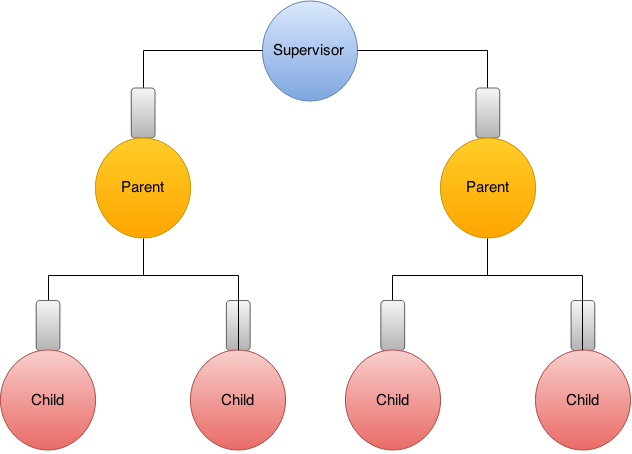
\includegraphics[scale=0.4]{images/tools/ActorModel.png} 
	\caption{Actor Model}
	\label{fig:ActorModel}
\end{figure}
\subsubsection{Actor Model}
The key points of the Actor model is building a hierarchy of  actors that receive messages in their mailbox. Figure \ref{fig:ActorModel} shows the general idea of the actors. The actors have a supervisor that will deliver tasks/messages to their inbox. The actors will then process the messages from their inbox and perform the appropriate task for each message. 
\subsubsection{Akka Actors}
The Actors in Akka are defined by Akka as lightweight, concurrent entities that use an event driven receive loop to process messages in its mailbox. An actors main functions can be boiled down to either receiving or sending messages. Akka's official documentation state that the size of a single actor is 300KB. With 1GB of heap memory, we can create approximately 2.5 million actors. 

These actors may share a thread or operate on different threads. We as developers do not need to worry about this as it is handled by the toolkit. A
\\\\
The way the actors determine the appropriate response to a message is by using pattern matching. Pattern matching in short allows us to check if the given message conforms to a certain pattern. This matching can be on the type of the message (int, string, boolean etc.) or on the actual value of the message (1, “text”, true). By using this we can raise abstraction on how an actor will operate. Pattern matching greatly reduces the clutter that many ``if'' statements can create. This will benefit us greatly when we implement our solution. 
\\\\
Another great benefit we get from Akka is its ability to change state, much like we would expect a protocol to. It can changes its state to simulate the state of the protocol. This allows us better understand how our actor will operate through its life cycle.
\begin{figure}[h]
	\centering
	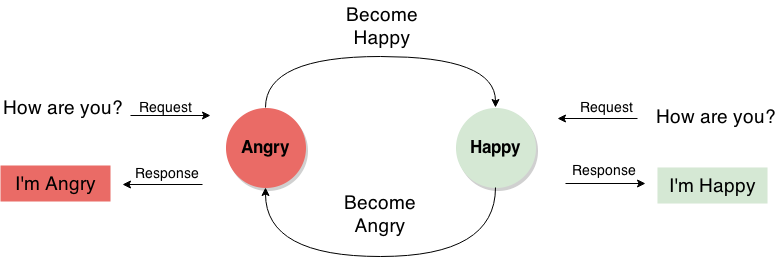
\includegraphics[scale=0.45]{images/tools/ActorState.png} 
	\caption{Actor State showing response to messages}
	\label{fig:ActorState}
\end{figure}
A simple state transition between ``Happy'' and ``Angry'' can be seen in figure \ref{fig:ActorState}. Depending on the state the actor is in, it will respond with a diffrent message.

%REF:
%Scala Booker http://www.artima.com/pins1ed/a-scalable-language.html 
%Actor Model http://ieeexplore.ieee.org/xpls/abs_all.jsp?arnumber=886427&tag=1

